%\acresetall
\chapter{Evaluation}\label{ch:chapter4}

In this chapter, we present the evaluation of \codeft{ferify}. In the first section, we validate our design of \codeft{ferify}. Next, we explain the tests we performed to verify that \codeft{ferify} has the results we expected. These tests covered typical use cases in which \codeft{ferify} can be employed. Finally we perform some tests to evaluate the performance overhead and the degree to which our solution impacts overall system usability.

\section{Validation}\label{sec:validation}

\par In Section~\ref{sec:overview} we discussed why \codeft{ferify} is secure. To expand on this and confirm that our claim is correct, we will present the security challenges we identified and tried to solve during the implementation of \codeft{ferify}. We can classify them by the permission level required to perform certain malicious operations on the running \ac{OS}. 

\subsection{Ring 3 Operations}

\par The ring 3 operations include all the actions an attacker can perform in the user space. Assuming that the attacker has gained \codeft{root} access, these actions include modification of system configuration files and executables to serve certain purposes for the attacker. 
\par The \codeft{ferify} process can be employed to overcome the challenge of how to protect the \ac{OS} at the ring 3 level from a malicious \codeft{root} user. By adding critical system files in the \acp{SACL} along with the correct permissions, we can \emph{deny} write access to any user, \emph{including} the \codeft{root} user. Depending on the security risk that is anticipated, the administrator must decide which files are critical. To ensure some of our assumptions, a few basic files we assessed needed protection are \codeft{/etc/passwd, /etc/shadow, /etc/pam.d/su}. Tests for these cases are covered in the next section.

\subsection{Ring 0 Operations}\label{sub:ring0}

\par File operations are performed by the kernel through system calls. The kernel can be modified only by the \codeft{root} user and, therefore, kernel memory can be accessed only while operating in ring 0 in the following ways:

\begin{itemize}
	\item System calls
	\item Kernel modules
	\item Kernel compilation and loading
	\item Kernel bugs
\end{itemize}

\par Generally, the system call \ac{API} is well defined and difficult to exploit. System call attacks usually target the system call table to modify the address of the system call functions with others of the attacker's choosing. However, to do that the attacker needs to be able to load kernel modules. So, this type of attack already falls into the second category, that of the kernel modules.

\par Everything is within reach when an attacker manages to load a kernel module. The module is running as part of the kernel, in ring 0, and has access to every physical and virtual resource available on the system. Kernel modules have access to and are able to modify all kernel functions and structures. There are protection mechanisms, like module digital signing, but all these checks are running on the same privilege level. To protect the guest \ac{OS} from that category
%category vs. type (CDP)
of attacks, which can also result in the installation of \emph{root-kits}, we trap and block the \codeft{init\_mod()} and \codeft{finit\_mod()} system calls;
%end sentence and then: By blocking the use of kernel module system calls we make module loading impossible. (CDP)
%, which make module loading possible, \emph{denying} it this way impossible.
by blocking the use of kernel module system calls we make module loading impossible.

\par To protect against a modified kernel, we took a simple approach that is easily implemented with \codeft{ferify}: initially we blocked the system call \codeft{kexec\_load()}.\footnote{This system call is used to load a new kernel for later execution.} In addition to that, we can detect the kernel files that are used to boot the system and write-protect them from all users. Also, in case of a reboot, the configuration will shut down the \ac{VM}, so automatically running on a modified kernel is prohibited. Aside from these protection measures, we decide not to expand further on this specific attack vector; there are already solutions, like vTPM~\cite{perez2006vtpm}, which implement a more sophisticated way of securing the system's boot procedure and verifying that the code launched by firmware is trusted. 

\par The kernel of an \ac{OS} is a program, and, as such, some bugs are typically expected: some might simply just crash parts of the kernel without any other consequences, but some can potentially be used to manipulate kernel memory structures and contents, or generally allow arbitrary code execution. These types of attacks require a very deep knowledge of the intricate Linux kernel to work successfully. Security patches are rolled out frequently to fix or secure against these bugs. We assessed these attacks to be out of the scope of this research, as the Linux kernel is constantly evolving. 

\section{Testing}\label{sec:testing}

\par We want to assess whether the files we protect with \codeft{ferify} are secure and cannot be accessed, except from those we have allowed in the \acp{SACL}. To assess that \codeft{ferify} worked as intended, we assume two basic scenarios. The first is that a remotely-connected authorized user should be able to work as before; we wanted \emph{usability} at the user level to remain unchanged. The second scenario is that of a hacked user account in which the attacker has remote access to the target \ac{VM} through exploitation of a vulnerability in the guest \ac{OS}. In this second case, we assume a ``worst case scenario'' in which the attacker has gained \codeft{root} privileges. 

\par As all higher-level programs and attacks eventually resort to the execution of  system calls, we create an environmental setup to assess all the test cases relevant to the system calls we trapped, in order to observe the behavior of the system and whether it conformed to expectations. We perform specific commands, as explained later, on the guest \ac{VM} to emulate the actions of an attacker. These commands reflect the cases when \codeft{ferify} could be applied and correspond to the most basic commands one can issue. 

\par The configuration includes two user accounts in the \emph{sudoers} group: one \emph{authorized} and one hacked by an \emph{attacker}. The hacked account is assumed to have become a sudoer through malicious actions. Additionally we create a group that includes both users, with the intention of assessing the per group policy enforcement to file access. The intent is to check detection of the illegal escalation of the hacked account to \codeft{root} and the effect this has. A high-level overview of our design is illustrated in Figure~\ref{fig:attack}. 

\par We also try, as \codeft{root}, to access files that were being protected from this specific user. These files include the \codeft{/etc/shadow} and \codeft{/etc/pam.d/su}, which were included in the \acp{SACL} to protect our initial \ac{VM} configuration.

\par By themselves these cases cover the basic set of actions that \codeft{ferify} was initially designed to monitor. Any combination of them is handled separately from the underlying \ac{OS}, reducing our problem to these elementary cases and making it easier to monitor and handle.

\begin{figure}[ht]
	\centering
	\begin{tikzpicture}
\small
\node[anchor= north west, fill=red!20, rectangle, rounded corners, draw=black, minimum width=30mm, minimum height=5mm, label={[yshift=-0.55cm]north:Vulnerable VM}] at (0, 0) {};


\node[anchor= north west, fill=blue!30, rectangle, rounded corners, draw=black, minimum width=30mm, minimum height=45mm, label={[yshift=-0.5cm]north:Trusted Zone}] at (4, -0.5) {};

\node[anchor= north west, fill=blue!20, rectangle, rounded corners, draw=black, minimum width=20mm, minimum height=8mm, label={[yshift=-0.8cm, align=center, font=\scriptsize]north:LibVMI /\\DRAKVUF}] at (0.5, -1.25) {};

\node[anchor= north west, fill=blue!20, rectangle, rounded corners, draw=black, minimum width=25mm, minimum height=8mm, label={[yshift=-0.75cm, align=center, font=\footnotesize]north:Ferify plugin}] at (4.25, -1.5) {};



\draw[anchor= south west, draw=red!70, line width=0.5mm,->] (2.5, 0.5) -- (2.5, 0);    
\node[anchor= north west, minimum width=5mm, minimum height=7mm,  label={[yshift=0cm, xshift=-0.25cm, align=center, font=\scriptsize ]north:Attacker}] at (2.5, 0.5) {};

\node[anchor= north west, minimum width=20mm, minimum height=8mm, label={[yshift=-0.7cm, align=center, font=\scriptsize]north:File Operation}] at (-0.5, -0.5) {};

\draw[anchor= south west, draw=blue!70, line width=0.5mm,->] (0.5, 0.5) -- (0.5, 0);
\node[anchor= north west, minimum width=5mm, minimum height=7mm,  label={[yshift=0cm, xshift=-0.25cm, align=center, font=\scriptsize ]north:Authorized user}] at (0.5, 0.5) {};

\draw[anchor= south west, draw=black, line width=0.3mm,->] (1.5, -0.5) -- (1.5, -1.25);
\draw[anchor= south west, draw=black, line width=0.3mm,->] (2.5, -1.75) -- (4.25, -1.75);
\node[anchor= north west, minimum width=20mm, minimum height=8mm, label={[yshift=-0.3cm, xshift=0.5cm, align=center, font=\scriptsize]north:Trapped\\ syscalls}] at (1.6, -1.5) {};

%\draw[anchor= south west, draw=black, line width=0.3mm,<-] (1.5, -2.5) -- (1.5, -2.2) -- (4.25, -2.2);
%\node[anchor= north west, minimum width=20mm, minimum height=8mm, label={[yshift=-0.45cm, xshift=0.25cm, align=center, font=\scriptsize]north:Yes / No}] at (1.9, -1.8) {};

\node[anchor= north west, minimum width=20mm, minimum height=8mm, label={[yshift=-0.35cm, align=center, font=\scriptsize]north:No}] at (-0.25, -2.5) {};

\node[regular polygon, regular polygon sides=8, minimum width=1cm, draw, line width=1pt](n1) at (-0.1, -2.8){};
\node[regular polygon, regular polygon sides=8, minimum width=1cm, draw=white,fill=red!80,label=center:\color{white}{\scriptsize\bfseries\sffamily STOP}]at(n1) at (-0.1, -2.8){};
%\node[anchor= north west, minimum width=20mm, minimum height=8mm, label={[yshift=-0.48cm, xshift=-0.35cm, align=center, font=\scriptsize]north:Block}] at (-0.75, -1.5) {};

\node[anchor= north west, minimum width=20mm, minimum height=8mm, label={[yshift=-0.35cm, align=center, font=\scriptsize]north:Yes}] at (0.25, -3.3) {};
\node[inner sep=0pt] (russell) at (1.75,-3.7)
    {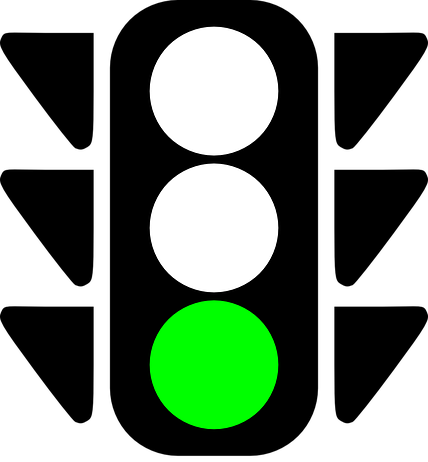
\includegraphics[width=.4cm]{figs/traffic-light2.png}};

%\draw[anchor= south west, draw=black, line width=0.3mm,<-] (4, -2.05) -- (4, -2.5);
%\draw[anchor= south west, draw=black, line width=0.3mm,->] (5, -2.05) -- (5, -2.5);

\draw[anchor= south west, draw=black, line width=0.3mm,->] (5, -2.3) -- (5, -2.6);

\draw[anchor= south west, draw=black, line width=0.2mm,-] (5, -2.6) -- (5.45, -2.9) -- (5, -3.2) -- (4.55, -2.9) -- (5, -2.6);
\draw[anchor= south west, draw=black, line width=0.3mm,->] (5, -3.2) -- (1.5, -3.2) -- (1.5, -4);
\draw[anchor= south west, draw=black, line width=0.3mm,->] (4.55, -2.9) -- (0.38, -2.9);

%%%%%%%%%%%%%%%%%%%%%%%%%%%%%%%%%%%%%%%%%%%%%%%%%

\node[anchor= north west, fill=white, rectangle, rounded corners, draw=black, minimum width=30mm, minimum height=30mm, label={[yshift=-0.5cm]north:HDD}] at (0, -4) {};
  
\node[anchor= north west, fill=white, rectangle, draw=black, minimum width=5mm, minimum height=7mm, label={[yshift=-0.5cm]north:}] at (0.2, -4.8) {};
\node[anchor= north west, fill=white, rectangle, draw=black, minimum width=5mm, minimum height=7mm, label={[yshift=-0.5cm]north:}] at (0.3, -4.9) {};
\node[anchor= north west, fill=white, rectangle, draw=black, minimum width=5mm, minimum height=7mm, label={[yshift=-0.5cm]north:}] at (0.4, -5) {};
\node[anchor= north west, fill=white, rectangle, draw=black, minimum width=5mm, minimum height=7mm,  label={[yshift=-1.5cm, xshift=-0.15cm, align=center, font=\scriptsize ]north:Other\\files}] at (0.5, -5.1) {};

\node[anchor= north west, fill=blue!30, rectangle, draw=black, minimum width=5mm, minimum height=7mm, label={[yshift=-0.5cm]north:}] at (2, -4.8) {};
\node[anchor= north west, fill=blue!30, rectangle, draw=black, minimum width=5mm, minimum height=7mm, label={[yshift=-0.5cm]north:}] at (2.1, -4.9) {};
\node[anchor= north west, fill=blue!30, rectangle, draw=black, minimum width=5mm, minimum height=7mm, label={[yshift=-0.5cm]north:}] at (2.2, -5) {};
\node[anchor= north west, fill=blue!30, rectangle, draw=black, minimum width=5mm, minimum height=7mm,  label={[yshift=-1.5cm, xshift=-0.15cm, align=center, font=\scriptsize ]north:Protected\\files}] at (2.3, -5.1) {};


\draw[anchor= south west, draw=black, line width=0.3mm,->] (6, -2.3) -- (6, -3.7);

\draw[fill=blue!20] (6, -4.1) ellipse (0.3cm and 0.1cm);
\draw[fill=blue!20] (6, -4) ellipse (0.3cm and 0.1cm);
\draw[fill=blue!20] (6, -3.9) ellipse (0.3cm and 0.1cm);
\node[anchor= north west, minimum width=7mm, minimum height=1mm , label={[yshift=-1cm, xshift=0.05cm, align=center, font=\small]north:SACL}] at (5.6, -3.7) {};
\draw[fill=blue!20] (6, -3.8) ellipse (0.3cm and 0.1cm);

\draw[anchor= south west, draw=black, line width=0.1mm,-] (5.7, -3.8) -- (5.7, -4.1);
\draw[anchor= south west, draw=black, line width=0.1mm,-] (6.3, -3.8) -- (6.3, -4.1);
  

\end{tikzpicture}
	\caption{Testing and validation concept.}
	\label{fig:attack}
\end{figure} 

\par First, we test whether an illegal \codeft{root} escalation is possible; then we test the file operations including \emph{create, open, read, write, copy, move,} and \emph{delete}.

\subsection{Root Escalation}

\par One of the first actions of an attacker or malicious program is to try to escalate its privileges to that of the \codeft{root} account. One of the techniques commonly employed is to add the compromised user to the \emph{sudoers} group. To avoid such an exploitation, every time a trap gets caught by the hypervisor we check whether the user executing a \codeft{sudo} command is actually allowed to do so.\footnote{If a user is allowed to execute the \codeftfs{sudo} command, that is specified in the initial administrative setup of \codeftfs{ferify} for the specific \ac{VM}.} If the user is a legitimate \codeft{sudoer}, the flow of our plugin continues normally to check the validity of the file operation against the \acp{SACL}. If the user is \emph{not} supposed to have \codeft{sudo} privileges, the system calls trapped by \codeft{ferify} that get invoked then get canceled, denying the ability to perform any \codeft{sudo} commands. Figure~\ref{fig:sudo_deny} shows the result of trying to execute a \codeft{sudo} command that gets denied, while also notifying the hypervisor of the event as shown in Figure~\ref{fig:sudo_deny_not}.

\begin{figure}[ht]
	\centering
	\footnotesize{\fontfamily{qcr}\selectfont 
		\begin{lstlisting}
bob@aHVM-domU:~$ sudo ls
   sudo: unable to open /etc/sudoers: Bad address
   sudo: no valid sudoers sources found, quitting
   sudo: unable to initialize policy plugin
bob@aHVM-domU:~$
		\end{lstlisting}}
	\caption{Denying \emph{sudo}.}
	\label{fig:sudo_deny}
\end{figure}

\begin{figure}[ht]
	\centering
	\footnotesize{\fontfamily{qcr}\selectfont 
		\begin{lstlisting}
Warning: Process root identity corruption detected in task 
	1377! Is 0 and should be 1002. 
	Invalidating syscall.
[SYSCALL:   2] CR3:0x1afec000  , RDI: 0x7f2178a931f7 ,sudo 
	PID:1377 [0:1002] wants 0 access to file: 
	/etc/sudoers (mode:0)
		\end{lstlisting}}
	\caption{Denying \emph{sudo} notification on the hypervisor.}
	\label{fig:sudo_deny_not}
\end{figure}

\par In the same manner, the result of trying to change a user's password is shown in Figure~\ref{fig:passwd_deny}.

\begin{figure}[ht]
	\centering
	\footnotesize{\fontfamily{qcr}\selectfont 
		\begin{lstlisting}
bob@aHVM-domU:~$ passwd alice
   Enter new UNIX password:
   Retype new UNIX password:
   passwd: Authentication token manipulation error
   passwd: password unchanged
bob@aHVM-domU:~$
		\end{lstlisting}}
	\caption{Denying password change from \emph{root} account.}
	\label{fig:passwd_deny}
\end{figure}


\par Having solved the issue of malicious \codeft{root} access, we then need to validate the expected behavior for file access, regardless of \codeft{root} user request.

\subsection{Authorized User Operation}

\par A very important aspect of any security solution is its impact on \emph{usability} for the normal user. The implementation of a secure system that remains fully usable is always a challenge. In this test we evaluate whether authorized users could normally access and work on their files. To test the file operations we create two files, \codeft{file1} and \codeft{file2}, and check whether we can open, move, or overwrite them. In the \acp{SACL}, we have entries for three files to test whether the third file could be created. The permissions for the files on the guest \ac{OS} and the \acp{SACL} are explained in Table~\ref{fig:file_perms1}.

\begin{table}[ht]
	\centering
	\footnotesize
	\caption{File permissions for authorized user.}
	\label{fig:file_perms1}			
	\begin{tabular}{c|c|c|c|c|c|c|c|c|c}
		\toprule
		\textbf{File} 
			&\multicolumn{3}{c|}{\textbf{Owner}}
			&\multicolumn{3}{c|}{\textbf{Group}}
			&\multicolumn{3}{c}{\textbf{Others}}\\
			
		\textbf{Name} 
			& \textbf{Read} & \textbf{Write} & \textbf{Execute} 
			& \textbf{Read} & \textbf{Write} & \textbf{Execute} 
			& \textbf{Read} & \textbf{Write} & \textbf{Execute} \\
		\toprule
		\multicolumn{10}{c}{Guest \ac{OS}}\\
		\hline
		\scriptsize{\fontfamily{qcr}\selectfont file1 }			
			& \checkmark & \checkmark & - 
			& \checkmark & - & - 
			& \checkmark & - & - 	\\	
		\scriptsize{\fontfamily{qcr}\selectfont file2 }			
			& \checkmark & \checkmark & - 
			& \checkmark & - & - 
			& \checkmark & - & - 	\\	
		\scriptsize{\fontfamily{qcr}\selectfont file3 }			
			& \checkmark & \checkmark & - 
			& \checkmark & - & - 
			& \checkmark & - & - 	\\	

		\hline
		\multicolumn{10}{c}{Hypervisor User's \ac{SACL}}\\
		\hline
		\scriptsize{\fontfamily{qcr}\selectfont file1 }			
			& \checkmark & \checkmark & - 
			& \checkmark & - & - 
			& \checkmark & - & - 	\\	
		\scriptsize{\fontfamily{qcr}\selectfont file2 }			
			& \checkmark & \checkmark & - 
			& \checkmark & - & - 
			& \checkmark & - & - 	\\	
		\scriptsize{\fontfamily{qcr}\selectfont file3 }			
			& \checkmark & \checkmark & - 
			& \checkmark & - & - 
			& \checkmark & - & - 	\\	
		\bottomrule
	\end{tabular}
\end{table}

\par After running our test script\footnote{The source code of the test script is included in Appendix~\ref{app:A}.} to verify the ability to access the user's files normally, the results show that the files are accessible as expected in every mode (Figure~\ref{fig:results1}).

\begin{figure}[ht]
	\centering
	\footnotesize{\fontfamily{qcr}\selectfont 
		\begin{lstlisting}
$ ./file_tests file1 file2 file3
   Success: Opened file1 for reading by user alex. Able to copy.
   Success: Opened file1 for writing by user alex.
   Success: file2 created by user alex.
   Success: user alex deleted file2.
   Success: user alex moved file1 to file3.

		\end{lstlisting}}
	\caption{File operations execution for authorized user.}
	\label{fig:results1}
\end{figure}

\par All basic file operations are available to an authorized user. We assess that the usability level for a normal user remains unchanged. By modifying the \ac{SACL} permissions, we can allow or deny certain operations on user- or group-owned files, according to the desired policy to be enforced.

\subsection{Attacker Operation - \codeft{root} Access - Immutable Objects}

\par One of the biggest problems in information security is that a \codeft{root} user or \codeft{administrator} of the system has access to \emph{all} its files and folders. That is the reason most attacks try to result in escalation of privileges to an administrative account. While the administrator is usually someone trusted and should have access to all \ac{OS} files for management issues, there are cases when even that person should not get access to certain information. The \codeft{ferify} process can provide the capability for normal users to have full access to their files, while at the same time the administrator cannot have full or even limited access to them. By setting the relevant file permissions, as per Table~\ref{fig:file_perms_root}, we can deny total access to the administrator on any file. This \ac{SACL} is different from the previous one, allowing for user-based policy.

\begin{table}[ht]
	\centering
	\footnotesize
	\caption{File permissions for root.}
	\label{fig:file_perms_root}			
	\begin{tabular}{c|c|c|c|c|c|c|c|c|c}
		\toprule
		\textbf{File} 
		&\multicolumn{3}{c|}{\textbf{Owner}}
		&\multicolumn{3}{c|}{\textbf{Group}}
		&\multicolumn{3}{c}{\textbf{Others}}\\
		
		\textbf{Name} 
		& \textbf{Read} & \textbf{Write} & \textbf{Execute} 
		& \textbf{Read} & \textbf{Write} & \textbf{Execute} 
		& \textbf{Read} & \textbf{Write} & \textbf{Execute} \\
		\toprule
		\multicolumn{10}{c}{Guest \ac{OS}}\\
		\hline
		\scriptsize{\fontfamily{qcr}\selectfont file1 }			
		& \checkmark & \checkmark & - 
		& \checkmark & - & - 
		& \checkmark & - & - 	\\	
		\scriptsize{\fontfamily{qcr}\selectfont file2 }			
		& \checkmark & \checkmark & - 
		& \checkmark & - & - 
		& \checkmark & - & - 	\\	
		\scriptsize{\fontfamily{qcr}\selectfont file3 }			
		& \checkmark & \checkmark & - 
		& \checkmark & - & - 
		& \checkmark & - & - 	\\	
		\hline
		\multicolumn{10}{c}{Hypervisor root's \ac{SACL}}\\
		\hline
		\scriptsize{\fontfamily{qcr}\selectfont file1 }			
			& - & - & - 
			& - & - & - 
			& - & - & - 	\\	
		\scriptsize{\fontfamily{qcr}\selectfont file2 }			
			& - & - & - 
			& - & - & - 
			& - & - & - 	\\	
		\scriptsize{\fontfamily{qcr}\selectfont file3 }			
			& - & - & - 
			& - & - & - 
			& - & - & - 	\\	
		
		\bottomrule
	\end{tabular}
\end{table}

\par After running our test script to verify the ability to deny access to \codeft{root} on the user's files, the results (Figure~\ref{fig:results2}) show that the files are inaccessible in every mode expected, according to the permissions we set in the \ac{SACL}. We assess that denying file access to the \codeft{root} user is an important security implementation, as it provides great \emph{confidentiality} assurance, as well as nullifying a range of attack vectors on systems, old or new.

\par A result of \codeft{ferify} is that it can be used to create immutable files on a system. With write access denied to everyone, there can be files that cannot be modified yet remain accessible for reading, providing great \emph{integrity} assurance.

\begin{figure}[ht]
	\centering
	\footnotesize{\fontfamily{qcr}\selectfont 
		\begin{lstlisting}
$ sudo ./file_tests file1 file2 file3
   Failure: Could not open file1 for reading by user root. 
            Cannot copy.
   Failure: Could not open file1 for writing by user root.
   Failure: file2 could not be created by user root.
   Failure: user root could not delete file2.
   Failure: user root could not move file1 to file3.

		\end{lstlisting}}
	\caption{File operations execution for non-authorized user.}
	\label{fig:results2}
\end{figure}


%\par One of the issues in the Linux file access permission system is that if a file belongs to a group, all users in that group can access the file, given the \ac{ACL} allows it. There are cases when a user wants to protect a file from being accessed but cannot, because other users belong to the same group, or multiple groups can access the file. 

%\par For this setup we created a third user \emph{jim}, who belongs only to the group \emph{alice} and a file owned by user and group \emph{alice}. There are two configurations available in the case of group access. User \emph{bob} belongs also to group \emph{alice} as a secondary group. Therefore, in this case all three users \emph{alice, bob, jim} have access to the file. By adding an entry to the \ac{SACL} for the file, with permissions \emph{rw-r-----} or \emph{640}, we effectively can deny access to anyone who belongs to group \emph{alice} as a secondary group, in this case user \emph{bob}. The results of the read operation for \emph{bob} and \emph{jim} show in fig. \ref{fig:sec_group_deny}

%\begin{figure}[ht]
%	\centering
%	\footnotesize{\fontfamily{qcr}\selectfont 
%		\begin{lstlisting}
%bob@HVM-domU:~$ more /home/alice/file_in_group_alice
%more: cannot open /home/alice/file_in_group_alice: 
%	Bad address
%
%jim@HVM-domU:~$ more /home/alice/file_in_group_alice
%Bob should not read this...
%		\end{lstlisting}}
%	\caption{Denying access from secondary group users}
%	\label{fig:sec_group_deny}
%\end{figure}
%
%\par By changing the permissions of the file to \emph{rw-------} or \emph{600} we deny access to everyone except for the actual owner of the file, in this case \emph{alice}. The same setup can be accomplished directly by changing the permissions of the file, but by using this solution, we can confuse the attackers, since it seems that they should have access as a group user. Now, not even user \emph{jim} has access to the file, although he should, as shown in fig. \ref{fig:group_deny}
%
%\begin{figure}[ht]
%	\centering
%	\footnotesize{\fontfamily{qcr}\selectfont 
%		\begin{lstlisting}
%jim@HVM-domU:~$ more /home/alice/file_in_group_alice
%more: cannot open /home/alice/file_in_group_alice: 
%	Bad address
%		\end{lstlisting}}
%	\caption{Denying access from group users}
%	\label{fig:group_deny}
%\end{figure}

\subsection{Malware Protection}

\par To make \codeft{ferify} work as a white-listing security application we implement a slightly different logic for the \codeft{execve()} and \codeft{execveat()} system calls. The results of our testing are satisfactory, but more thorough testing should be performed. 

\par We have successfully managed to apply different execution permissions and block application execution on a \emph{per-user} level. This differs from the other system call's handling in that \emph{if} the executable \emph{is not} in the \ac{SACL}, we \emph{deny} execution. There is no different \ac{SACL} implementation for this case, just separate handling of the \codeft{execve()} system call. Since we assume that the system is secure when we launch \codeft{ferify}, any file in the filesystem should not be malicious. For a malware to create a persistence mechanism, it will have to write executable code on the victim system and run it at some point. Since that file will not be in the \ac{SACL}, we automatically block that executable from running, thus having efficiently mitigated a large attack-vector of malware. To mitigate against attacks that modify \ac{OS} executables with malicious ones, system executables should also be marked as \emph{non-writable} in the \acp{SACL} to prevent modification and ensure their \emph{integrity}.

\subsection{Append-only Mode}

\par Once attackers have achieved system penetration, they start accessing the \ac{OS} in many ways; accessing of files for information gathering, creation of persistence mechanisms, and installation of back-doors are just a few. To remain undetected they must ``hide their tracks''; attackers usually edit system logs to erase their presence. Log files are created by appending entries at the end of the file, but this is not an enforced file-access policy. As such, log files are generally accessible to and editable by attackers. Forcing log files to be writable only at the end of the file can prevent attackers from hiding their tracks.

\par Due to the \ac{OS} limitations, we could not enforce partial write permissions on a file. Given the permissions the user requests, a file can be opened only in its entirety. The \codeft{ferify} process is capable of enforcing a write-only access policy to files and attackers are not able to open a file in read-write mode, select, and delete the log entries that reveal their presence. Attackers would have to blindly delete entries or empty the entire log, actions that should be noticed by the system administrator. We believe that this policy can be proven to be a substantial hindrance to malicious actors trying to ``cover their tracks'' in the system.

\section{Performance Overhead}\label{sec:performance}

In this section we present the performance overhead observed on the guest \ac{OS} when running \codeft{ferify}. To have a baseline for comparison, we created a \codeft{Python} script\footnote{The source code of the performance test script is included in Appendix~\ref{app:B}.} that performs some of the trapped system calls and measures the execution time. From the results we calculated the average execution time of each system call and the standard deviation. We then performed time-execution measurements in three stages: The first was under normal \ac{CPU} scheduling preferences. For the second run, we set the \codeft{niceness} of \codeft{ferify} to \codeft{-20}. \emph{Niceness} for Linux is how favorable the scheduling will be for the process, with \codeft{-20} being the best value and \codeft{10} the normal value. Finally, for the third run, in conjunction with changing the niceness of the process, we additionally set the \ac{I/O} niceness to the best available value. This changes the \ac{I/O} scheduling of processes, giving \codeft{ferify} \ac{I/O} priority over all others. Initially, we timed the execution of the script over a number of iterations without running \codeft{ferify} to extract an average time that we will use as a reference. Figure~\ref{fig:script} shows the three commands we used to run \codeft{derify} with different priorities.

\begin{figure}[ht]
	\centering
	\footnotesize{\fontfamily{qcr}\selectfont 
		\begin{lstlisting}
$ sudo ./ferify
$ sudo nice -n -30 ./ferify
$ sudo nice -n -30 ionice -c 1 -n 0 ./ferify
	\end{lstlisting}}
	\caption{\codeft{Ferify} priority command-line settings.}
	\label{fig:script}
\end{figure}


\subsection{Hypervisor - \ac{VM} Switch}

\par As mentioned in Subsection~\ref{sub:invm}, one of the most intense operations in virtualization is the switch between the hypervisor and the \ac{VM}. \ac{CPU} virtualization extensions improve with every new model release, but this switch is still significant. To measure this overhead in performance, we ran \codeft{ferify} with empty \acp{SACL}. This way, \codeft{ferify} trapped the appropriate system calls and performed the switch between the \ac{VM} and the hypervisor. Because the \acp{SACL} were empty, there was insignificant computation performed while on the hypervisor, almost immediately switching back to the \ac{VM}. 

\par Table \ref{tbl:measure1} shows the results and the performance overhead of the \ac{VM} context-switch. As expected, the cost of VM-exit and VM-entry is significant. 

\begin{table}[ht]
\centering
\caption{Context-switch performance overhead measurements.}
\label{tbl:measure1}
\begin{tabular}{c|cc|cc|c}
	\toprule
	& \multicolumn{2}{c|}{With \codeft{ferify}} 
	& \multicolumn{2}{c|}{Without \codeft{ferify}}
	& \\
	System call 		& Avg time (msec) & Std dev & Avg time (msec) & Std dev & Increase \\	
	\toprule
	\multicolumn{6}{c}{No scheduler priority set}\\
	\hline
	\codeft{open()} 	& 1.410575 & 0.042011 & 0.272977 & 0.040227 & 516.74\%\\
	\codeft{rename()} 	& 1.177306 & 0.060151 & 0.119034 & 0.032872 & 989.05\%\\
	\codeft{unlink()} 	& 1.265741 & 0.044768 & 0.110438 & 0.022926 & 1,146.11\%\\
	\hline
	\multicolumn{6}{c}{With best \codeft{nice} value}\\
	\hline
	\codeft{open()} 	& 1.808050 & 0.118523 & 0.272977 & 0.040227 & 662.34\%\\
 	\codeft{rename()} 	& 1.510058 & 0.114244 & 0.119034 & 0.032872 & 1,268.59\%\\
	\codeft{unlink()} 	& 1.617183 & 0.116488 & 0.110438 & 0.022926 & 1,464.34\%\\	
	\hline
	\multicolumn{6}{c}{With best \codeft{nice} and \codeft{ionice} values}\\
	\hline
	\codeft{open()} 	& 1.763718 & 0.131143 & 0.272977 & 0.040227 & 646.10\%\\
	\codeft{rename()} 	& 1.547484 & 0.111831 & 0.119034 & 0.032872 & 1,300.03\%\\
	\codeft{unlink()} 	& 1.648374 & 0.120758 & 0.110438 & 0.022926 & 1,492.58\%\\	
	\bottomrule
\end{tabular}	
\end{table}


\subsection{\ac{SACL} Performance Overhead}

\par The information for the files in the \acp{SACL} is stored in a hash table. The index of the table is the pathname. Since the lookups made in the hash table depend on the depth of the file's directory tree, the searching of a file in the \ac{SACL} is of \emph{O(d)} complexity, where \codeft{d} is the aforementioned depth. Since the depth of a directory tree is usually relatively short, we assess the algorithm to be efficient. To verify the claim that the search time does not depend on the entries of the \ac{SACL}, we ran the same test with the same settings and files, but with different \ac{SACL} sizes each time (as shown in Table~\ref{tbl:measure}). To avoid as much \ac{OS} interference as we could, we set both settings of \codeft{niceness} to the best value. The results seem to support our claim; the average execution time of the tested system calls is of the same magnitude. 

\begin{table}[ht]
\centering
\caption{Hash-table search times (msec).}
\label{tbl:measure}
\begin{tabular}{ c | c | c | c | c }
	\toprule
	& \multicolumn{4}{c}{\ac{SACL} size} \\
	System call & 100 & 1,000 & 10,000 & 100,000 \\	
	\toprule
	\codeft{open()} & \tab0.203920\tab & \tab0.204899\tab & \tab0.206650\tab & \tab0.202786\tab \\
	\codeft{rename()} 	& 0.256427 & 0.256371 & 0.259813 & 0.255484 \\
	\codeft{unlink()} 	& 0.191526 & 0.193019 & 0.194595 & 0.190740 \\
	\bottomrule
\end{tabular}	
\end{table}

\par Despite the promising results, we needed to measure \codeft{ferify}'s total performance overhead when running on a full filesystem. To evaluate \codeft{ferify}'s efficiency, we ran the same script as before, but with a full filesystem \ac{SACL} containing more than 400,000 entries. For the purposes of testing, our \ac{VM} had no extra programs installed and we had created just a few user files. In a normally used \ac{OS} many more entries would be expected.

\par Although the increase in execution time seems extremely large, the average execution time of a single system call seems to remain within usable limits. While using the guest \ac{VM} to evaluate the use experience, we did not notice any delays. 

\par Table \ref{tbl:measure2} shows the result of the second run of our test. We observed that the total performance overhead remained in the same magnitude. Some numbers might seem contradictory, but this is normal as the Linux kernel schedules each running process differently and continuously creates more. This is the reason we focused on the magnitude instead of the actual numbers. Compared to the dominant cost of switching between the hypervisor and the guest \ac{VM}, we assessed that the hash-table implementation and the permission checking algorithm had an insignificant impact on performance. This is the exact reason we decided to trap each system call individually, instead of trapping the system call handler, which is the kernel's entry point to all system calls. This case would cause even greater overhead, as the \ac{VM} context switch would happen for \emph{each and every} system call invoked by \emph{all} processes running on the \ac{OS}. 

\makeatletter
\setlength\@fptop{0\p@}
\makeatother

\begin{table}[ht]
\centering
\caption{\codeft{ferify}'s performance overhead measurements.}
\label{tbl:measure2}
\begin{tabular}{c|cc|cc|c}
	\toprule
						& \multicolumn{2}{c|}{With \codeft{ferify}} 
						& \multicolumn{2}{c|}{Without \codeft{ferify}}
						& \\
	System call 		& Avg time (msec) & Std dev & Avg time (msec) & Std dev & Increase \\	
	\toprule
	\multicolumn{6}{c}{No scheduler priority set}\\
	\hline
	\codeft{open()} 	& 1.742811 & 0.064730 & 0.272977 & 0.040227 & 638.45\%\\
	\codeft{rename()} 	& 1.824321 & 0.059661 & 0.119034 & 0.032872 & 1,532.60\%\\
	\codeft{unlink()} 	& 1.627008 & 0.098494 & 0.110438 & 0.022926 & 1,473.24\%\\
	\hline
	\multicolumn{6}{c}{With best \codeft{nice} value}\\
	\hline
	\codeft{open()} 	& 1.743948 & 0.047873 & 0.272977 & 0.040227 & 638.86\%\\
	\codeft{rename()} 	& 1.776946 & 0.057694 & 0.119034 & 0.032872 & 1,492.80\%\\
	\codeft{unlink()} 	& 1.593204 & 0.047137 & 0.110438 & 0.022926 & 1,442.63\%\\
	\hline
	\multicolumn{6}{c}{With best \codeft{nice} and \codeft{ionice} values}\\
	\hline
	\codeft{open()} 	& 2.105518 & 0.101172 & 0.272977 & 0.040227 & 771.32\%\\
	\codeft{rename()} 	& 2.170908 & 0.155974 & 0.119034 & 0.032872 & 1,823.77\%\\
	\codeft{unlink()} 	& 1.919827 & 0.149137 & 0.110438 & 0.022926 & 1,738.38\%\\
	\bottomrule
\end{tabular}	
\end{table}



%\subsection{Large \ac{SACL} performance overhead}
%
%\par Adding more files to the \acp{SACL} may add a more substantial overhead. As shown in \ref{fig:pathname_length}, there is a significant amount of pathnames with lengths between 10 and 130. Having so many elements in a linked list introduces increased time in searching for a record. To assess the performance overhead we repeated the previous test, but this time after adding more than 1000 files in the \acp{SACL}. Writing \acp{ACL} for thousands of files is extremely time-consuming and error-prone. To automate this procedure we created a standalone script that pauses the guest \ac{VM}, mounts its filesystem to the hypervisor and starting from a specified mount-point, it returns the required information. 
%
%\par After having generated a \ac{SACL} that corresponds to the current guest \ac{OS} filesystem permissions, the administrator can easily modify the permissions to reflect the desired policy to be enforced. 
%
%\begin{figure}[ht]
%	\centering
%	%\begin{tikzpicture}
\begin{axis}[
title={Pathname length distribution of sample \ac{OS}},
xlabel={Pathname length},
ylabel={Count (thousands)},
xmin=0, xmax=600,
ymin=0, ymax=27000,
xtick={0,100,200,300,400,500,600},
ytick={0, 5000, 10000, 15000, 20000, 25000},
ymajorgrids=true,
xmajorgrids=true,
grid style=dashed,
]

\addplot[very thick, blue, smooth] table [
col sep=comma,
x = Length,
y = Count,
] {figs/graph1.csv};

\end{axis}
\end{tikzpicture}
%	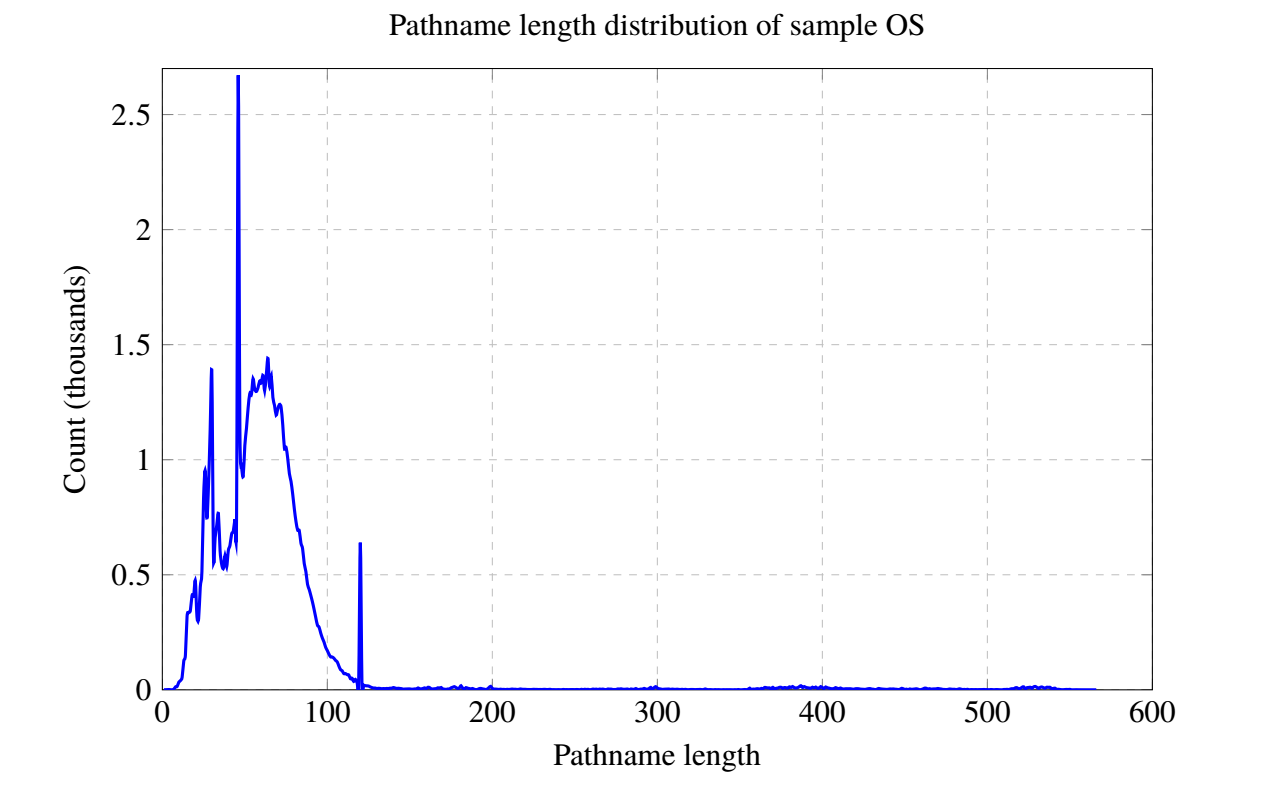
\includegraphics[scale=0.45]{images/graph1.png}
%	\caption{Pathname length count}
%	\label{fig:pathname_length}
%\end{figure}
%
%
%\subsection{Full \ac{OS} \ac{SACL} performance overhead}
%
%\par Finally, we wanted to evaluate whether \emph{Ferify} can be used on the whole filesystem of a guest \ac{OS}. To do that we just created a \ac{SACL} that was generated by the aforementioned script when providing as mount-point the root folder of the guest \ac{OS}. Since the vast majority of the files is in the same range of length, we expect significant delays in our script execution.
%



